%%%% PLEASE REPLACE ENTIRELY WITH YOUR OWN CONTENT %%%%

\ifcase\doclanguage
\or
  \chapter[Estat de l'art]{Estat de l'art de la tecnologia utilitzada o aplicada en aquest TFG}

  El capítol «Estat de l'Art de la Tecnologia» ofereix una visió detallada dels avenços actuals relacionats amb el tema del vostre treball. Hauria de descriure les teories, models, algorismes clau o desenvolupaments de programari i maquinari, recolzats per articles revisats per experts i altres recursos com ara llibres, patents, informes tècnics, etcètera. Aquest capítol estableix el context i ajuda els lectors a entendre el panorama existent en el camp. En conseqüència, les \textbf{cites a referències bibliogràfiques rellevants} són una part important del contingut.
  
  Aquest capítol no només ha de resumir la recerca existent, sinó que també ha de fer-ne una \textbf{avaluació crítica}. Això implica destacar les llacunes o limitacions en la tecnologia actual per preparar el terreny per a les tasques que el TFG abordarà. Al final del capítol els lectors haurien de tenir una comprensió clara del que ja se sap sobre el tema, del que encara queda per aprendre i de com el TFG contribueix a aquesta «conversa acadèmica» en curs.

  \section{Internet of Medical Things (IoMT)} 

  Aquí teniu un parell de cites a referències sobre \LaTeX~\cite{latexcompanion} i electrodinàmica \cite{einstein}.

  L’Internet of Medical Things (IoMT) representa una evolució natural dins l’ecosistema de l’Internet de les Coses (IoT), aplicat específicament al sector sanitari. Aquest concepte engloba una xarxa de dispositius mèdics connectats que recopilen, processen i transmeten dades clíniques en temps real amb l’objectiu de millorar l’atenció mèdica, optimitzar la gestió hospitalària i afavorir la monitorització remota dels pacients. Entre els dispositius més habituals dins l’IoMT trobem monitors cardíacs, pulsòmetres, inhaladors intel·ligents, implants connectats, sistemes de dosificació automatitzada de medicació etc.
  El creixement de l’IoMT ha estat exponencial els darrers anys, impulsat per l’avenç tecnològic, la miniaturització de sensors, la proliferació de la connectivitat sense fils i la necessitat d’una atenció sanitària més eficient i personalitzada. Cada vegada els hospitals estàn adoptant mès aquestes tecnologíes I s’espera que aquesta tendència es mantingui en creixement en els pròxims anys. Tanmateix, aquesta mateixa expansió comporta un augment significatiu de la superfície d’exposició a ciberatacs. A mes a mès, s’espera que a mida que avança la seva adopció, aquests dispositius tingun rols mès determinants en les tasques mèdiques, la qual cosa pot implcar una major criticitat en cas de ciberatac. 
  A diferència dels sistemes informàtics convencionals, els dispositius IoMT sovint operen en entorns amb recursos computacionals limitats (processador, memòria, energia), i moltes vegades han estat dissenyats amb una orientació funcional, no pas de seguretat. Això els fa especialment vulnerables a atacants que poden aprofitar configuracions per defecte, manca d’actualitzacions, credencials febles o vulnerabilitats en els protocols de comunicació. A més, la connexió d’aquests dispositius mitjançant xarxes Wi-Fi o altres canals inalàmbrics exposa el sistema a atacs com l’escolta (sniffing), suplantació de dispositius (spoofing), atacs de denegació de servei (DoS) entre altres. 
  Un dels aspectes més crítics del risc en entorns IoMT és la naturalesa de les dades que gestionen. Les dades mèdiques són altament sensibles, personals i sovint irreversibles en cas de filtració. Un accés no autoritzat pot vulnerar drets fonamentals com la privacitat i tenir conseqüències legals greus per a les institucions sanitàries. 
  En aquest context, la ciberseguretat en l’àmbit IoMT no es pot considerar un afegit posterior al desplegament dels sistemes, sinó un requisit fonamental des de la fase de disseny. Això, és especialment rellevant en entorns on les conseqüències d’un atac poden tenir un impacte directe sobre la salut i la seguretat física dels pacients.
  Finalment, és important destacar que la protecció dels sistemes IoMT també ha de ser escalable i adaptable. L’amenaça no és estàtica, i els vectors d’atac evolucionen constantment. Davant d’aquesta realitat, la recerca en ciberseguretat per a l’IoMT s’està orientant cada cop més cap a solucions dinàmiques, com ara sistemes intel·ligents basats en aprenentatge automàtic que permetin detectar patrons anòmals de comportament i actuar de forma proactiva. En aquest sentit, la generació de datasets reals que simulin tant trànsit legítim com maliciós en entorns IoMT esdevé una peça clau per entrenar i validar aquestes solucions emergents.

  \section{Message Queuing Telemetry Transport (MQTT)}
  El Message Queuing Telemetry Transport (MQTT) és un protocol de missatgeria lleuger dissenyat per a la comunicació entre dispositius amb recursos limitats i connexions de xarxa poc fiables o amb amplada de banda reduïda. Aquest protocol s’ha convertit en un estàndard de facto en moltes aplicacions IoT, inclòs l’àmbit de l’Internet of Medical Things (IoMT), per la seva eficiència, simplicitat i facilitat de desplegament. Desenvolupat originalment per IBM l’any 1999, MQTT segueix un model de comunicació publish/subscribe, que afavoreix la desconnexió temporal dels nodes i la minimització de l’ús de xarxa, dos requisits habituals en xarxes IoT.
  En una arquitectura MQTT, el component central és el broker, un servidor que actua com a intermediari entre els dispositius que publiquen dades (publishers) i els que les reben (subscribers). Els dispositius no es comuniquen directament entre ells, sinó que ho fan a través del broker, que rep els missatges publicats en un tema determinat (topic) i els redirigeix als clients que s’han subscrit a aquest tema. Aquesta arquitectura desacoblada simplifica el disseny de sistemes escalables i resilients.
  A l’àmbit IoMT, aquesta estructura és especialment útil per gestionar sensors mèdics que generen dades de manera periòdica, com ara nivells de glucosa, senyals d’electrocardiograma (ECG), o mesures de tensió arterial. Aquests sensors poden publicar lectures de manera eficient al broker MQTT, i altres components del sistema (com bases de dades, aplicacions clíniques o sistemes d’alerta) poden consumir aquesta informació segons les seves necessitats.
  
  El protocol MQTT opera habitualment sobre la pila TCP/IP, utilitzant el port 1883 per a connexions no segures i el port 8883 quan es fa servir TLS (Transport Layer Security) per protegir la transmissió. Tot i que també existeixen adaptacions que funcionen sobre WebSockets, el transport TCP és el més comú en entorns de comunicació entre dispositius embeguts.
  Entre les característiques tècniques més destacades d’MQTT, podem ressaltar:
  \begin{itemize}
      \item \textbf{Qualitat del servei (QoS):} MQTT ofereix tres nivells de fiabilitat en el lliurament de missatges, cosa que permet ajustar el comportament segons els requisits de l’aplicació.
      \item \textbf{Retenció i missatges persistents:} Un missatge es pot marcar com a retained perquè quedi emmagatzemat al broker i sigui enviat automàticament als nous subscriptors del topic. Això permet garantir que les dades més recents estiguin disponibles en tot moment, encara que el dispositiu que les va enviar originalment ja no estigui actiu.
      \item \textbf{Sessions persistents:} MQTT pot mantenir estat entre connexions. Quan un client es desconnecta, pot conservar la seva subscripció i reprendre la comunicació amb normalitat quan es torni a connectar, gràcies al paràmetre clean session
      \item \textbf{Protocol lleuger:} Amb una capçalera mínima de només 2 bytes, MQTT genera molt poca sobrecàrrega, cosa que el fa extremadament eficient per dispositius amb CPU limitada, poca memòria RAM o connexions de xarxa inestables o intermitents.
      \item \textbf{Model desacoblat (publish/subscribe):} Els clients no necessiten conèixer ni l’adreça ni l’estat dels altres dispositius. Això facilita l’escalabilitat i la flexibilitat del sistema, ja que els rols de publicador i subscriptor poden canviar dinàmicament.
      \item \textbf{Jerarquia de temes (topics):} Els topics MQTT segueixen una estructura jeràrquica (p.e., hospital/room3/patient5/oximeter), i és possible fer subscripcions amb comodins (+, #), fet que proporciona una gran flexibilitat però també pot ser explotat maliciosament si no es controla adequadament.
  \end{itemize}
  Malgrat aquests avantatges, el protocol MQTT no està pensat amb la seguretat com a objectiu principal, cosa que el fa vulnerable en entorns crítics com l’IoMT si no s’hi afegeixen mecanismes de protecció. Les principals limitacions de seguretat inclouen:
  \begin{itemize}  
      \item \textbf{Manca d’autenticació forta:} MQTT defineix només un sistema bàsic d’autenticació mitjançant username i password, sense mecanismes d’autenticació mútua ni suport nadiu per a protocols d’identitat moderna (com OAuth 2.0). Si el canal de comunicació no es protegeix amb TLS/SSL, tant les dades com les credencials es transmeten en text pla, fet que les fa extremadament vulnerables a atacs man-in-the-middle i sniffing.
      \item \textbf{Control d’accés deficient:} En moltes implementacions, si no es configuren polítiques d’ACL (Access Control List), qualsevol client pot publicar o subscriure’s a qualsevol tema. Això permet a un atacant llegir dades confidencials, injectar informació falsa o llançar atacs com el topic hijacking (suplantació de canals legítims).
      \item \textbf{Broker com a punt crític:} El broker MQTT és un únic punt de fallada. Si és compromès o queda saturat, tota la infraestructura de comunicació es veu afectada. Això el fa vulnerable a atacas de denegació de servei o DdoS. 
      \item \textbf{Flooding i sobrecàrrega:} Un client maliciós pot publicar un gran volum de missatges en bucle o utilitzar QoS elevat per generar trànsit excessiu. Si el broker no disposa de mecanismes de limitació o filtrat, pot ser fàcilment col·lapsat.
      \item \textbf{Lack of message integrity:} Si no s’usa TLS, tampoc hi ha garanties que els missatges no hagin estat modificats durant el trànsit. Això obre la porta a atacs de manipulació de dades que poden tenir greus conseqüències en entorns mèdics.
  \end{itemize}
  Donada la seva extensió en entorns IoT i les seves característiques adaptades a dispositius amb recursos limitats, MQTT s’ha triat com a protocol principal per a la simulació de trànsit en aquest treball. El seu ús permet generar escenaris tant de comunicació legítima com maliciosa, en els quals es poden observar comportaments anòmals mitjançant eines d’anàlisi i detecció. Això facilita la creació de datasets realistes per a l’entrenament d’IDS basats en IA.
    
  \begin{figure}[ht]
    \centering
    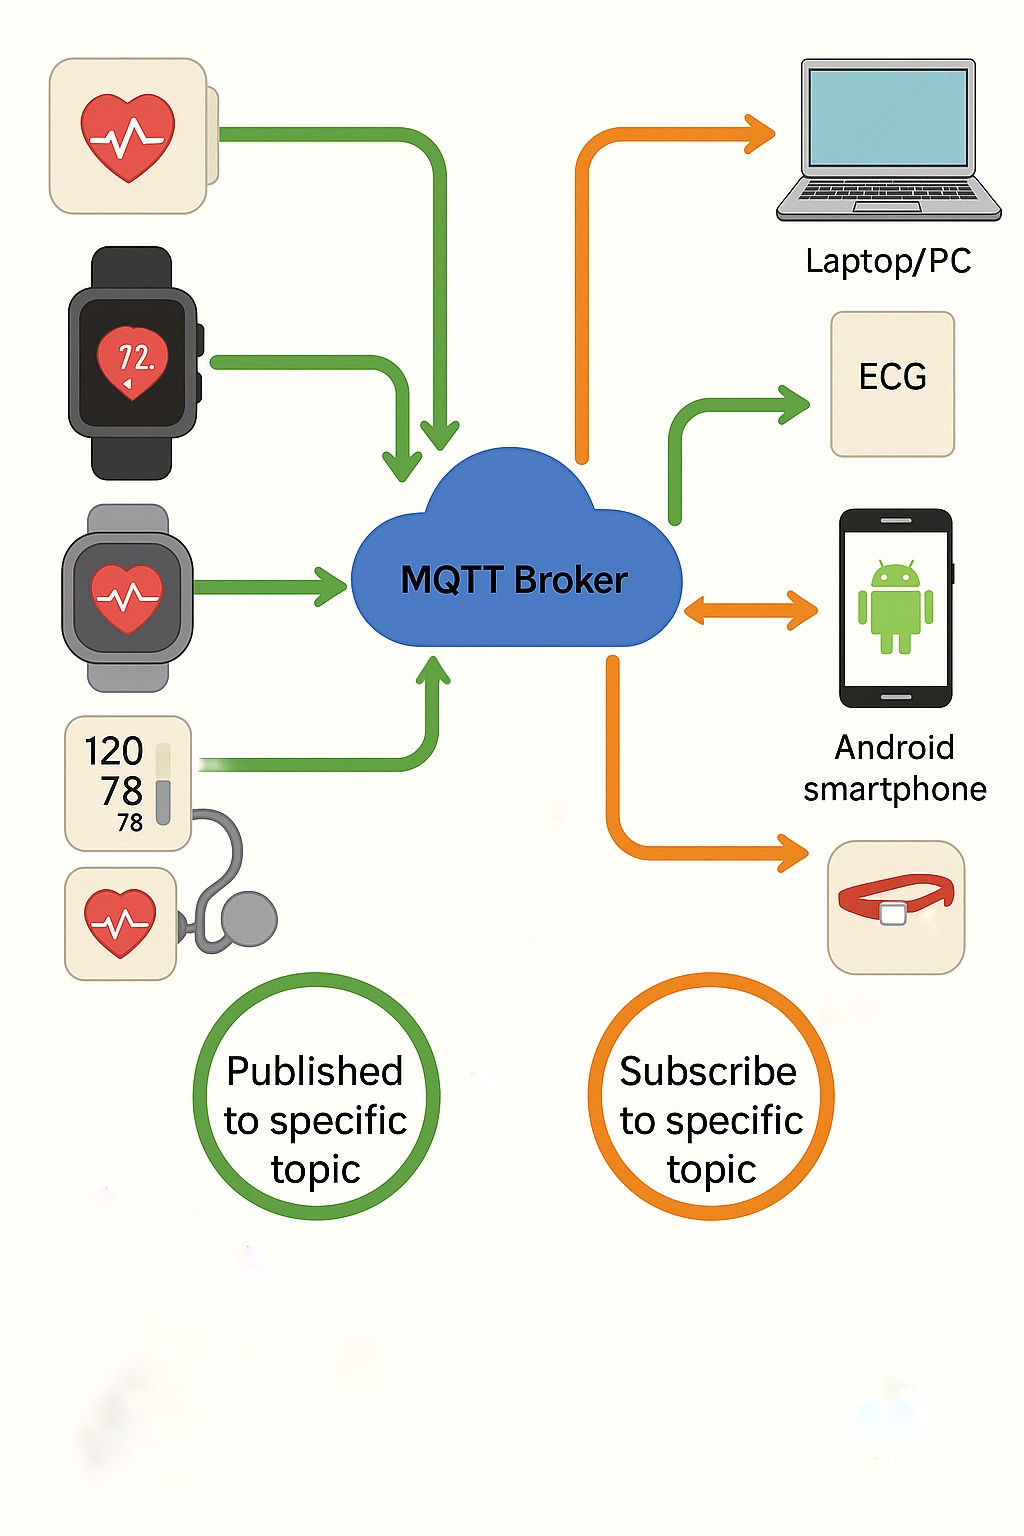
\includegraphics[width=0.4\textwidth]{img/MQTT_IoMT.jpg}
    \caption{Protocol MQTT en un entorn IoMT. Adaptat de \cite{mqttfig}.}
    \label{fig:MQTT}
  \end{figure}

  \section{Altres protocols en l'entorn IoMT}
  Pel que fa a altres protocols, tot i que MQTT és el protocol principal emprat en aquest treball, també es considera l’ús del protocol Constrained Application Protocol (CoAP) com a alternativa o complement en la generació de trànsit. CoAP és un protocol pensat específicament per a dispositius amb recursos limitats en xarxes IoT. Funciona sobre UDP, cosa que li proporciona una latència molt baixa i un comportament lleuger, tot i que això també comporta certes limitacions pel que fa a la fiabilitat de la transmissió.
  CoAP segueix un model client-servidor similar a HTTP però optimitzat per a entorns embeguts. Utilitza mètodes com GET, POST, PUT i DELETE, i permet observar recursos mitjançant un sistema d’actualitzacions automàtiques (observe). A diferència de MQTT, que és orientat a un model (publish/subscribe), CoAP és més adequat per a interaccions puntuals o consulta de recursos puntuals.
  En aquest treball, l'ús de CoAP es contempla per generar variabilitat en els escenaris de comunicació i per comparar comportaments de trànsit entre protocols amb estructures diferents. Això pot enriquir el dataset resultant i millorar la capacitat de generalització del sistema d’IA per a la detecció d’intrusions.
  
  En l’entorn mèdic, també son utilitzats altres protocols d’aplicació com HTTP/HTTPS o bé Extensible Messaging and Presence Protocol (XMPP) I també protocols de capa física Bluethoot Low Energy (BLE), Near Filed Communication (NFC) o bé dades celulars com NB-IoT que no seràn utilitzats en aquest treball. 
\or
  \chapter[Estado del arte]{Estado del arte de la tecnología utilizada o aplicada en este TFG}

  El capítulo «Estado del Arte de la Tecnología» ofrece una visión detallada de los avances actuales relacionados con el tema de vuestro trabajo. Debería describir las teorías, modelos, algoritmos clave o desarrollos de software y hardware, respaldados por artículos revisados por expertos y otros recursos como libros, patentes, informes técnicos, etcétera. Este capítulo establece el contexto y ayuda a los lectores a entender el panorama existente en el campo. En consecuencia, las \textbf{citas a referencias bibliográficas relevantes} son una parte importante del contenido.
  
  Este capítulo no solo debe resumir la investigación existente, sino que también debe hacer una \textbf{evaluación crítica} de ella. Esto implica destacar las lagunas o limitaciones en la tecnología actual para preparar el terreno para las tareas que el TFG abordará. Al final del capítulo, los lectores deberían tener una comprensión clara de lo que ya se sabe sobre el tema, de lo que aún queda por aprender y de cómo el TFG contribuye a esta «conversación académica» en curso.

  \section{Apartado 1}

  Aquí teneis un par de citas a referencias sobre \LaTeX~\cite{latexcompanion} y electrodinámica \cite{einstein}.

  \section{Apartado 2}
  \lipsum[7]

\else
  \chapter[State of the art]{State of the art of the technology used or applied in this thesis}

  The "Technology State of the Art" chapter offers a detailed view of the current advancements related to the topic of your work. It should describe key theories, models, algorithms, or developments in software and hardware, supported by peer-reviewed articles and other resources such as books, patents, technical reports, etc. This chapter sets the context and helps readers understand the existing landscape in the field. Consequently, the \textbf{citations to relevant bibliographic references} are an important part of the content.
  
  This chapter should not only summarize existing research but also provide a critical evaluation of it. This involves highlighting the gaps or limitations in current technology to set the stage for the tasks that the bachelor's thesis will address. By the end of the chapter, readers should have a clear understanding of what is already known about the topic, what still needs to be learned, and how the bachelor's thesis contributes to this ongoing "academic conversation."

  \section{Topic 1}

  Here you have a couple of cites to references about \LaTeX~\cite{latexcompanion} and electrodynamics \cite{einstein}.

  \section{Topic 2}
  \lipsum[7]

\fi



